\documentclass[]{article}   % list options between brackets
\usepackage{}              % list packages between braces
\usepackage[english]{babel}
\usepackage{graphicx}

\begin{document}

\title{Mario: A Machine Learning Classification Approach}   % type title between braces

\author{Erek Speed and Nick Villalva}         % type author(s) between braces
\date{December 6, 2011}    % type date between braces
\maketitle

\begin{abstract}
 The purpose of this project was to construct a 
\end{abstract}

\section{Introduction}     % section 1
This project is a departure from the common data sets of the machine learning world. The authors have eschewed corpi and proteins in lew of something a bit closer to their hearts.  To this end, we've repurposed the classification powers of the machine learning world for use with a classic platforming game from our youth, Super Mario Brothers(Mario).  Despite the levity of the topic, the discussion of the algorithms is just as reasonable as the common problems of the field.  Indeed, if we consider the Mario world a rough approximation of our own then it's easy to see the relevance of of studying a simpler version of what some might consider the holy grail of artificial intelligence: human level interaction with arbitrary environments.
\newline\newline
To that end, this end the work here explores treating world interaction as a classification problem.  Specfically, we want to classify every possible state of the world as a particular action. Taking such an action would lead to a new state and a new action.  By continuing in this fashion a agent explores the world in the manner it was trained.
\newline\newline
With such a vision, the present work describes and evaluates the application of popular machine learning algorithms to our lofty task.  We start with a discussion of the of previous work in the mario AI area.  In general, no standing body of data exists for Mario domain.  To overcome this obstacle we developed a system for a generating a dataset cooresponding to optimal actiosn in response to the current environment.  A description of this process and various attempted optimizations appears in \ref{sec:datagen}.  With data in hand, the authors attempt to create a Mario agent by applying popular machine learning algorithms to said data.  Each classifier is described in turn in section \ref{sec:class}.  \ref{sec:results} evaluates the previously described classifiers using common performance metrics as well as actual performance on unknown Mario levels.  We end with a discussion of future work and a conclusion.

\subsection{Division of Work}

\section{Previous Work}
\label{sec:prevwork}
The present work is the first to attemp to solve Mario as a classification problem.  That said, in recent years there has been a surge of attempts to develop Mario playing Agents.  The interest started with a MarioAI contest in 2009 which solicited all computer agent solutions to the Mario problem \cite{2}.  Interestingly, the report from said contest was dominated by handcoded such as A* \cite{3}.  In fact, due to the ability to reverse engineer the simulation engine the problem was reduced to a planning problem and easily solved.  A scattering of learning algorithms involving neural networks and genetic algorithms were submited but performed poorly.  Later, learning algorithms were given their own category in which they only had to learn a single level. With such a constraint, learning algorithms were able to reach near optimal performance \cite{me}. In contrast, we reject the notion that Mario is only solvable with complete prior knowledge of the the world.  We also acknowledge the vastness of the problem space and the failures of past learning problems getting lost in its many plateaus.  By creating an agent which trains on data generated from an expert player we greatly shink the problem space while maintaining some amount of generality.  



\section{Data Generation}     % section 2.1
\label{sec:datagen}

\section{Classifiers}
\subsection{Software}
\subsubsection{Libraries}
We considered several libraries for this project and ultimately settled on Java ML \cite{javaml}. Our main 
requirements were that it support the various classifiers we wished to use, have an implementation of feature 
selection, and be capable of interfacing with the Mario Benchmarking \cite{mariobenchmark} software. The 
Mario software was obtained from the MarioAI competition and is written in Java. It allows for the use of 
players that implement an Agent interface to take in data about the world and push buttons on the controller 
to move Mario as it sees fit. We looked at using weka \cite{weka}, Java ML \cite{javaml}, scikit-learn 
\cite{scikit}, and libsvm \cite{libsvm}. 

Weka is a relatively full featured library written in java, and as such was one of the most attractive libraries 
available. It is well used and contains all of the types of classifiers we hoped to use. The major drawback 
surrounding the use of weka was the data format it required. Programatically it was rather complicated to setup 
data on the fly, and translating the datafiles we had already created into the proper format was a taxing proposition. 

Scikit, written in python, was considered due to the ease of data manipulation in python and the fact that both 
of us were comfortable with the language. The major drawback of this is that we would have to find a way to 
export all of our classifiers and import them into the java based Mario Benchmarking software. The libsvm 
integration with scikit was very appealing and was one of the major reasons we considered it.

Libsvm was a great choice because its widespread use and its proficient handling of various multiclass support 
vector machines. What made us shy away from direct use of libsvm was that all three other libraries had wrappers 
for libsvm that would allow us to reap its benefits from within a single library that contained all of our classifiers.

We ultimately chose Java ML due to its simple data interface, native java compatibility, and the fact that it 
wrapped both Weka and libsvm functionality. This enabled us to use libsvm for our support vector classifiers, 
wrapped Weka classifiers for random forests, na\"{i}ve Bayes, KNN and REP trees, and forward and backwards feature 
selection. 

\subsection{KNN}
\subsubsection{Reasons for selection and expectations}
We chose to include k nearest neighbors as one of our algorithms because we thought that the large search space 
would help it identify similarities between attributes in our dataset. Hopes were high for the reduced feature 
sets as they should only be looking at the attributes that have an impact on the action to be taken for a given 
board configuration.  We expected KNN to train slowly and respond slowly, making it less than ideal for actual play. 
However, the simplicity of the algorithm would give us a good baseline for what is possible.

\subsubsection{Parameter selection}
KNN had very few parameters to select – the number, $k$, of neighbors to look at and the distance measure that would 
be used to find the nearest neighbors. First, due to the scarcity of data for some of our classes, we chose to 
experiment with $k$ from one to five. We then selected a few distance measures to test – Euclidian, symmetric uncertainty 
and Jaccard indexing. We then ran a grid search using five-fold cross validation to determine the best set. The metrics 
we measured to compare the success of classifiers with one another were accuracy, precision, f1 and recall. 


\subsection{Na\"{i}ve Bayes}
\subsubsection{Reason for selection and expectation}
Na\"{i}ve Bayes was an attractive classifier to use since it allowed for priors, allowed us to view a probability 
distribution on optimal actions, and yielded classifications relatively quickly. We expected it to perform decently 
with the full ensemble of data, but really shine with a reduced dataset that hopefully proved to have a better 
signal to noise ratio. 

\subsubsection{Parameter selection}
The wrapped implementation of na\"{i}ve Bayes provided by Java ML required very few parameters. We were given the 
option of using a Laplace correction as a prior and the use of logarithmic results. As our dataset was sparse, we 
were appreciative of the ability to make the classifier aware of this in order to improve performance. Due to the 
very limited number of parameters, our grid search for optimal parameters focused on whether or not to include a 
Laplace correction and the size of dataset on which the classifier was trained. 

\subsection{REP Trees}
\subsubsection{Reason for selection and expectation}
REP (Reduced Error Pruning) trees, while not specifically covered in class, were used as a representative of the 
various tree classsification methods. This algorithm builds a decision/regression tree and internally splits the 
dataset into folds in order to perform reduced error pruning. The key motivation for including REP trees in our 
ensemble of classifiers was to have a tree that actively prunes itself as they are purported to be especially good 
at classifying categorical data. We expected the tree to take longer to train than KNN or na\"{i}ve Bayes, but to 
respond to requests quickly.

\subsubsection{Parameter selection}
The REP tree algorithm we utilized required a few parameters -- the minimum number of records per leaf, the number 
of folds for pruning, and the maximum depth. Due to the size and imbalance of our data, we decided to retain most 
of the default settings of three folds, no maximum depth and two instances per leaf. Our experimentation with REP 
trees focused on the amount of data provided for training and its impact on the accuracy of the classifier.

\section{Results}
\subsection{Metrics}
In evaluating our methods we decided to use a combination of accuracy, precision, recall and f1 characteristics to 
evaluate our cross validation results for KNN, SVM and na\"{i}ve Bayes. As the tree algorithms do not measure these
statistics, we used root mean squared error as our metric.

Similarly, a metric was needed to compare results from runs through the Mario 
Benchmark. The metrics picked for that were a combination of a weighted fitness score that the benchmarking program 
calculated and a scalar progress count that represented how far through the level the classifier controlled Mario was 
able to get. The following analyses are based on these metrics.

\subsection{KNN}
\subsubsection{Cross Validation}
Running five-fold cross validation on KNN revealed interesting results. Cross validation revealed that 3 was the optimal
choice for $k$. The first thing we noticed was with respect to the distance measures -- Euclidean distance was worse than
the Jaccard index for out data. In cross validation, the best results achieved with Euclidean distance were precision of 0.645,
accuracy of .851, recall of .0327 and F1 measure of .0472. Due to many classes not being chosen, precision could not be averaged
across the datasets for a few configurations. The results are below.

\begin{table}[h!]
	\begin{center}
		\caption{Cross validation results for KNN}
		\begin{tabular}{l | l || l | l | l | l }
		Data Size & Feature Reduction & Precision & Accuracy & Recall & F1 Measure \\
		\hline
		20K & 99\% & 0.915 & 0.989 & 0.0597 & 0.0625 \\
		20K & 95\% & 0.920 & 0.990 & 0.0599 & 0.0625 \\
		20K & 90\% & 0.917 & 0.989 & 0.0598 & 0.0625 \\
		2.5K & 5x5 & 0.837 & 0.988 & 0.101 & 0.0957 \\
		2.5K & 5x5 & 0.882 & 0.991 & 0.101 & 0.0956 \\
		\hline
		\end{tabular}
	\end{center}
\end{table}

\subsubsection{Mario Benchmark}
As expected, the KNN algorithm was incredibly slow to respond to move requests. Additionally, as eluded to by the invalid precision
results on some of the cross validation, the majority of responses consisted of holding down the forward and jump buttons continually
in a manner that prevented Mario from doing more than one jump per level. As such, the KNN classifiers never finished a level. The best
performance of the classifier was on the simplest level on the lowest difficulty with a weighted fitness of 1488. It was able to make its
way through 26.9\% of the level.

\subsection{SVM}
\subsubsection{Cross Validation}
Cross validation for our support vector machines was done with two-fold validation, as the size of our datasets made 
it very costly time-wise to perform more than two-fold validation. A grid search was done for parameters using both linear
and RBF kernels. The best linear svm was produced by $C = .01$ with a score of $0.9842$, and the best RBF svm was produced by
$\gamma = .5$ and $C = 10$ with a score of $0.6999$.

\subsubsection{Mario Benchmark}
The performance of our trained SVMs on the benchmark was rather interesting. With data reduction of 99\% (the 1\% dataset), the support
vector machine was incapable of learning to pass the simplest level which requires running forward and jumping. It consistently
collided with a ledge and got stuck until time ran out. With data reductions of 95\% or less, the SVM was capable of learning to
run forward and jump repeatedly, allowing it to pass the simplest levels. The RBF svm identified by cross validation finished every
level that contained no gaps, enemies or blocks, and was capable of finishing the easiest level that included gaps. The linear svm
identified by cross validation was unable to complete a level in spite of its superior cross validation results. Behaviorally, it
never let go of the jump button and therefor Mario was unable to jump after his first hop.

\subsection{Na\"{i}ve Bayes}
\subsubsection{Cross Validation}
Cross validation of the various na\"{i}ve Bayes classifiers alerted us that it would not be a very good player. For an example of the
performance as evaluated by five-fold cross validation, the results for 20,000 datapoints with various levels of feature reduction are
shown below.

\begin{table}[h!]
	\begin{center}
		\caption{Cross validation results for Na\"{i}ve Bayes}
		\begin{tabular}{l | l || l | l | l | l }
		\hline
		Data Size & Feature Reduction & Precision & Accuracy & Recall & F1 Measure \\
		\hline
		20K & 99\% & 0.133 & 0.967 & 0.0751 & 0.0973 \\
		20K & 95\% & 0.077 & 0.931 & 0.0565 & 0.0935 \\
		20K & 90\% & 0.082 & 0.943 & 0.0617 & 0.0864 \\
		\hline
		\end{tabular}
	\end{center}
\end{table}

\subsubsection{Mario Benchmark}
Much like the linear svm, none of the nai\"{i}ve Bayes classifiers were able to complete a level on the benchmark. The highest fitness
value found was shared between four different parameter settings. Classifiers trained with the 5x5 dataset with both 5000 and 10,000
datapoints were capable of scoring a 1913 on the easiest level. Likewise, Classifiers trained on the 5\% and 1\% datasets with 20,000
datapoints achieved the same score.

This alludes to an interesting threshold difference between the reduced datasets and the 5x5 grid data. Reduced datasets required four
times as many datapoints to achieve the same level of success as the 5x5 grid with a Bayesian classifier. Intuitively this does not make sense,
as the length of the feature vectors in the 1\% and 5x5 datasets were about the same. 

\subsection{REP Trees}
\subsubsection{Cross Validation}
As previously mentioned, cross validation of REP trees was performed by measuring the root mean squared error. Using the various levels of feature
reduction and changing the number of folds used by the algorithm did not change this metric. This makes sense because it should choose the optimal
features to look at and use as few of them as possible. The root mean squared error of our REP trees was $0.0353$.

\subsubsection{Mario Benchmark}
REP trees were one of the few classifiers to successfully complete the clear levels with ledges consistently while showing the lowest threshold for
datapoints required to reach optimality. 

\begin{table}[h!]
	\begin{center}
		\caption{REP tree classifiers capable of scoring the highest score}
		\begin{tabular}{l | l || l  }
		\hline
		Data Size & Feature Reduction & Score \\
		\hline
		500 & 5x5 & 6568 \\
		500 & 95\% & 6568 \\
		500 & 90\% & 6568 \\
		\hline
		\end{tabular}
	\end{center}
\end{table}

Also of note is that with 99\% feature reduction, the REP trees were unable to complete the level. This suggests that a key feature for learning to 
rest between jumps is discarded with the move from 95\% to 99\%.

\subsection{Random Forests}
\subsubsection{Cross Validation}

\subsubsection{Mario Benchmark}

\subsection{Overall}

\begin{figure}
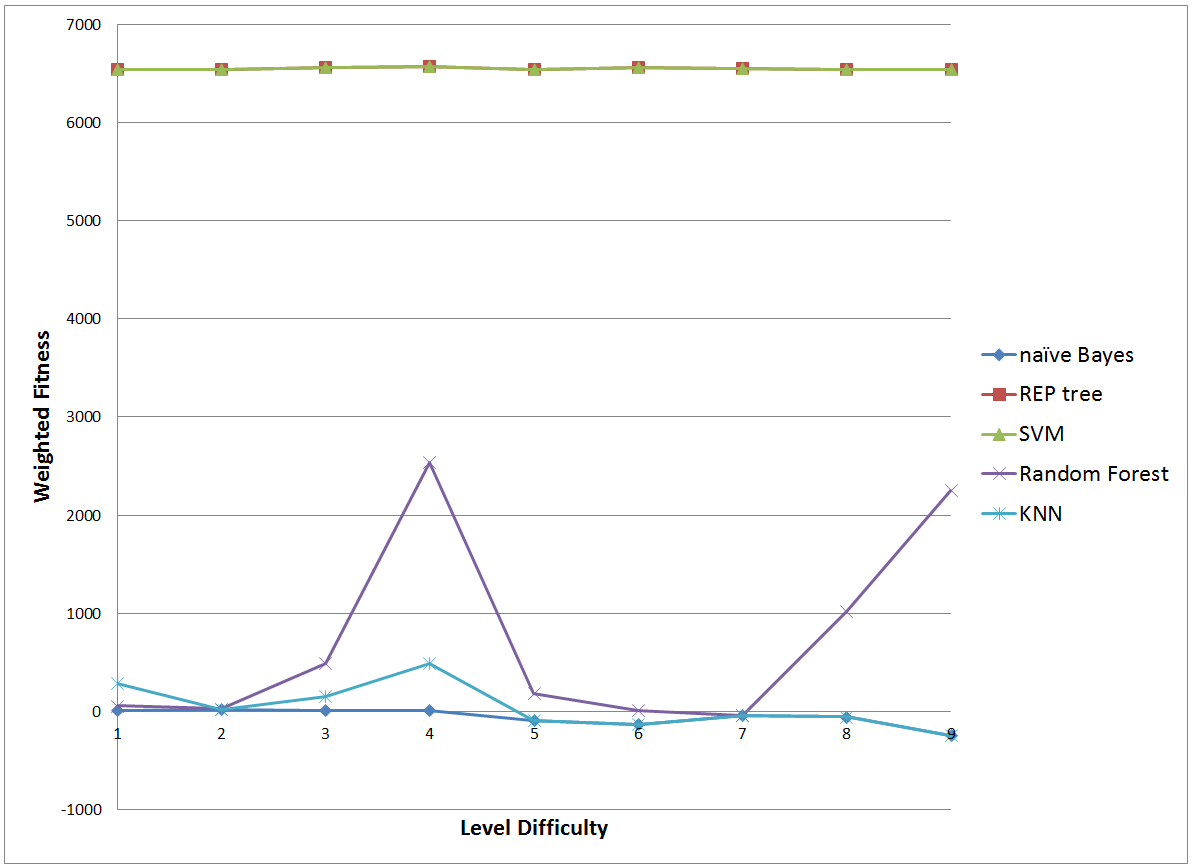
\includegraphics[width=110mm]{basic.png}
\caption{Graph of performance on basic levels by classifier}
\end{figure}

\begin{figure}
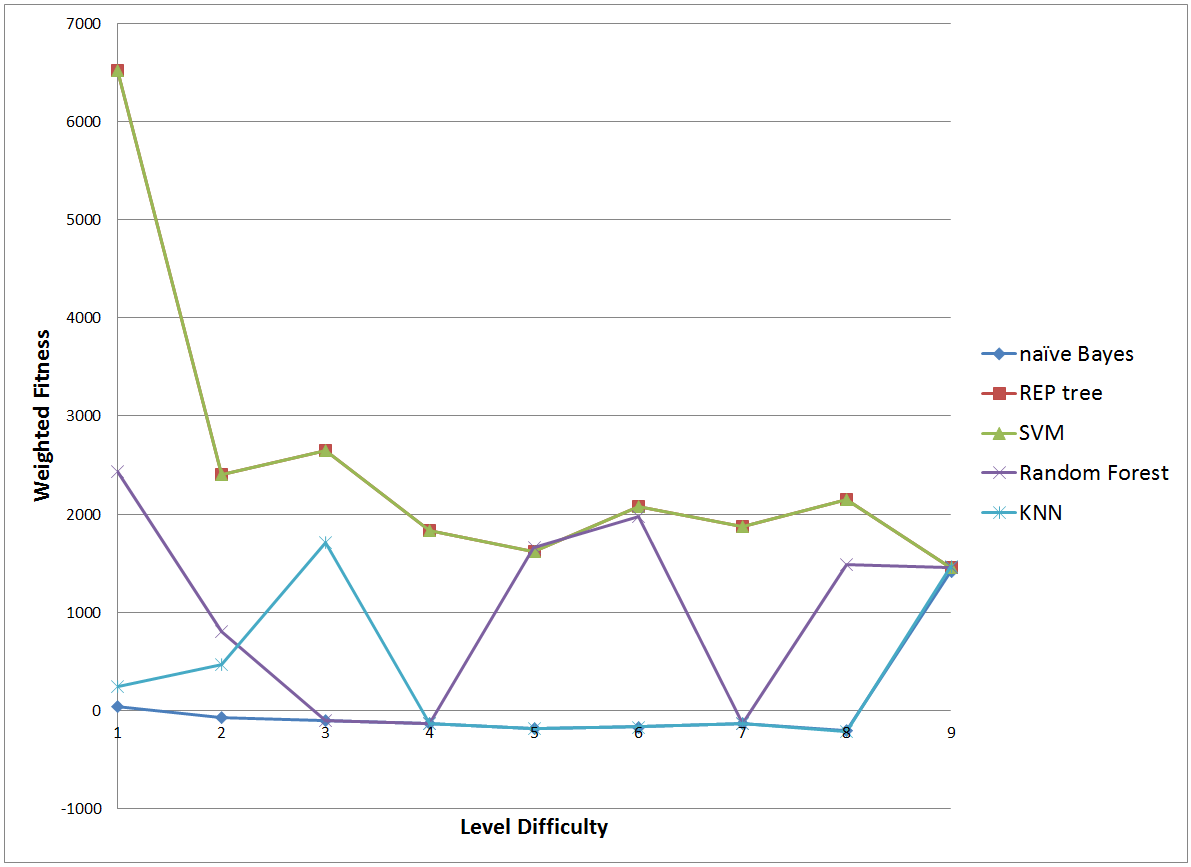
\includegraphics[width=110mm]{gaps.png}
\caption{Graph of performance on levels with gaps by classifier}
\end{figure}

\begin{figure}
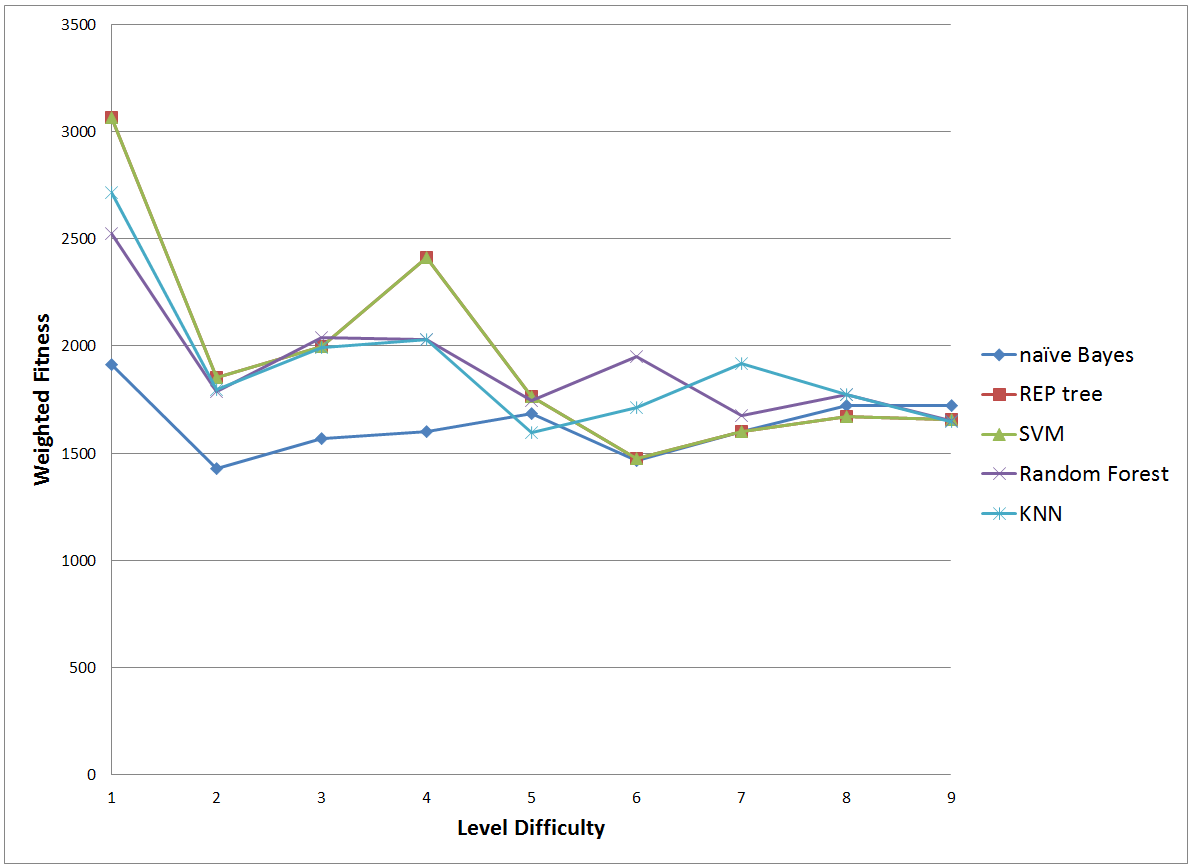
\includegraphics[width=110mm]{enemies.png}
\caption{Graph of performance on levels with enemies by classifier}
\end{figure}

\begin{figure}
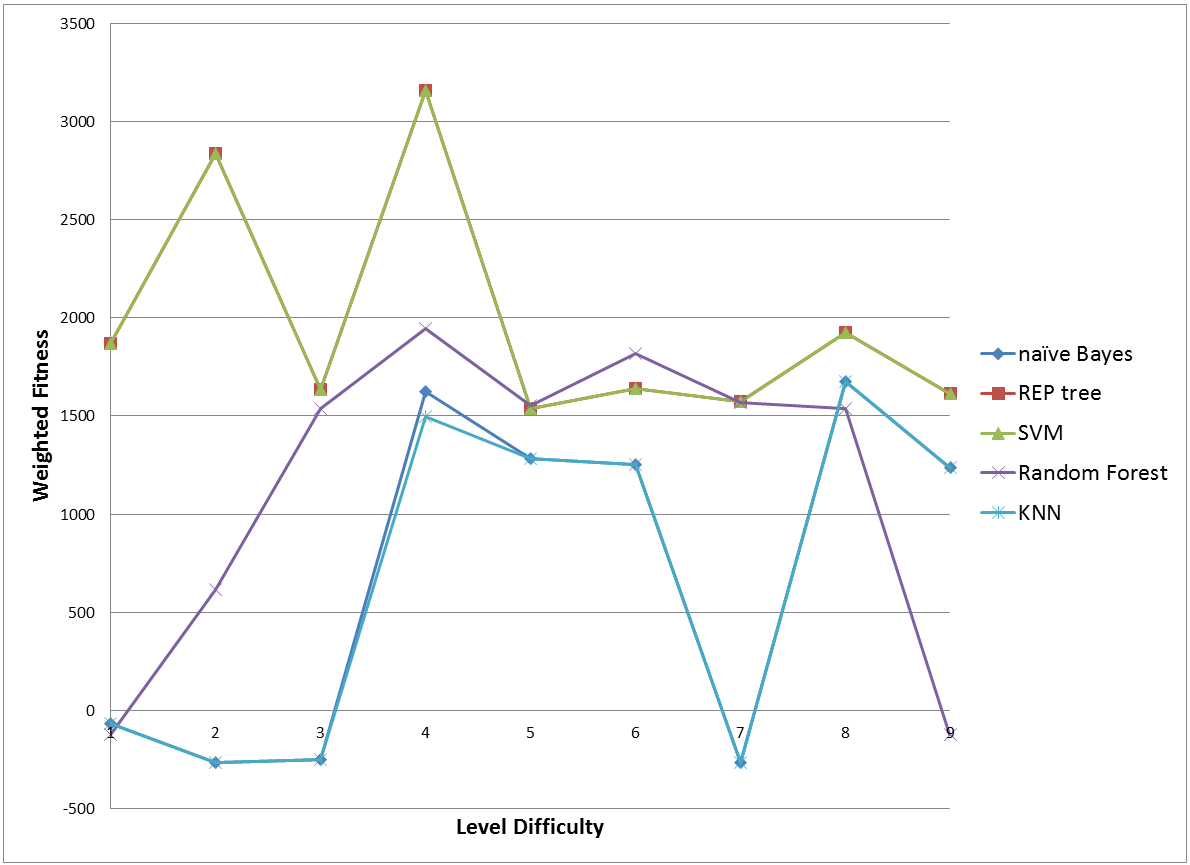
\includegraphics[width=110mm]{enemiesblocks.png}
\caption{Graph of performance on levels with enemies and blocks by classifier}
\end{figure}

\begin{figure}
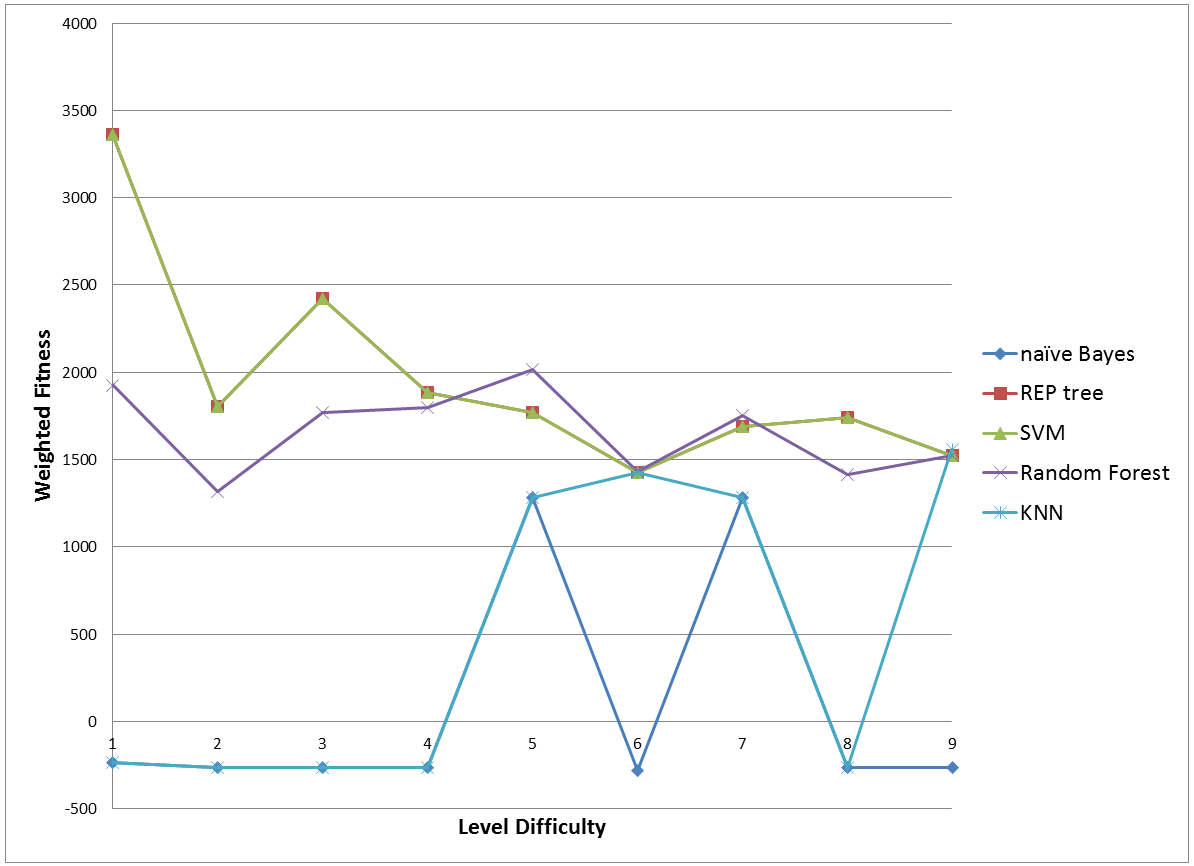
\includegraphics[width=110mm]{enemiesblocksgaps.png}
\caption{Graph of performance on levels with enemies, blocks and gaps by classifier}
\end{figure}

\section{Future Work}

\section{Conclusion}


\begin{thebibliography}{9}
  % type bibliography here
  \bibitem{javaml}
  Abeel, T.; de Peer, Y. V. \& Saeys, Y. Java-ML: A Machine Learning Library, Journal of Machine Learning Research, 2009, 10, 931-934
  \bibitem{mariobenchmark}
  http://www.marioai.org/
  \bibitem{weka}
  Mark Hall, Eibe Frank, Geoffrey Holmes, Bernhard Pfahringer, Peter Reutemann, Ian H. Witten (2009); The WEKA Data Mining Software: An Update; SIGKDD Explorations, Volume 11, Issue 1.
  \bibitem{scikit}
  scikit has a bibtex
  \bibitem{libsvm}
  libsvm has a bibtex
\end{thebibliography}

\end{document}
